\begin{figure}[!htbp]
	\centering
	\resizebox{\textwidth}{!}{%
		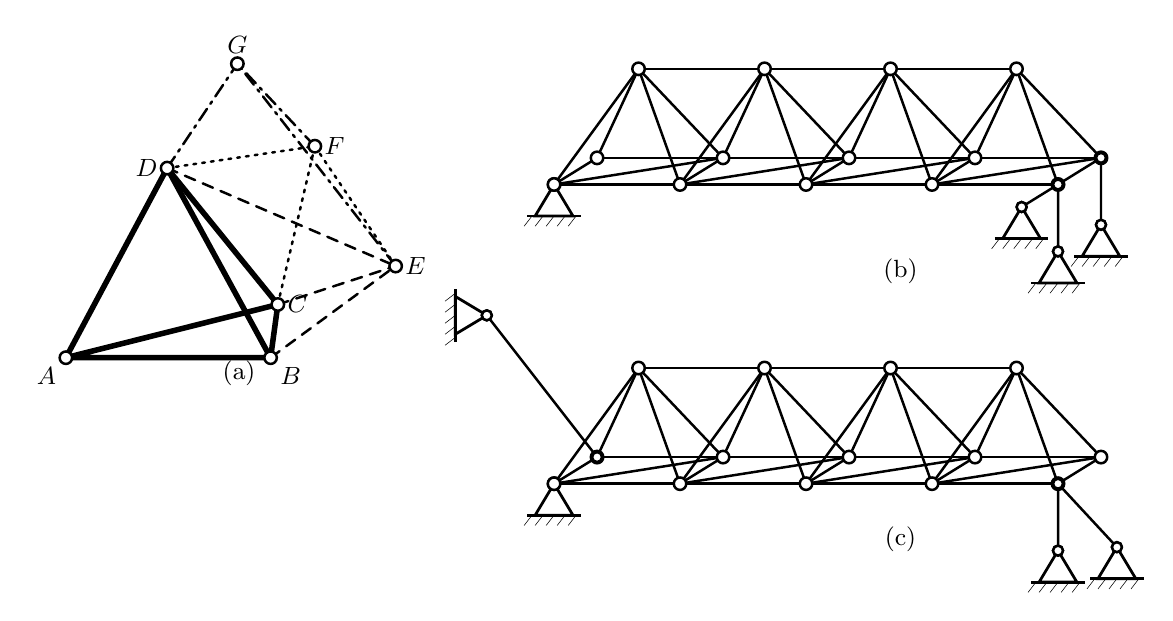
\begin{tikzpicture}[
			asta/.style={line width=0.9pt, line cap=round, line join=round, black},
			base/.style={line width=2.0pt, line cap=round, line join=round, black},
			nuova/.style={line width=0.9pt, line cap=round, line join=round, black,
				dash pattern=on 4pt off 3pt},
			futura/.style={line width=0.9pt, line cap=round, black,
				dash pattern=on 1pt off 2.2pt},
			quarta/.style={line width=0.9pt, line cap=round, black,
				dash pattern=on 5pt off 2.2pt on 1pt off 2.2pt},
			nodo/.style={circle, fill=white, draw=black,
				inner sep=0pt, minimum size=4.5pt, line width=0.9pt},
			etich/.style={font=\small},
			pan/.style={font=\small},
			assi/.style={x={(1cm,0cm)}, y={(0.42cm,0.26cm)}, z={(0cm,1cm)}},
			]
			
			%% simboli di vincolo --------------------------------
			\newcommand{\cerniera}[1]{%
				\begin{scope}[shift={(#1)}, x={(1cm,0cm)}, y={(0cm,1cm)}]
					\draw[line width=1.0pt](0,0)--(-0.24,-0.40)--(0.24,-0.40)--cycle;
					\draw[line width=1.0pt](-0.34,-0.40)--(0.34,-0.40);
					\foreach \x in {-0.28,-0.14,0.00,0.14,0.28}
					\draw[very thin](\x,-0.40)--++(-.10,-0.13);
			\end{scope}}
			\newcommand{\pareteSX}[1]{%
				\begin{scope}[shift={(#1)}, x={(1cm,0cm)}, y={(0cm,1cm)}]
					\draw[line width=1.0pt](0,0)--(-0.40,-0.24)--(-0.40,0.24)--cycle;
					\draw[line width=1.0pt](-0.40,-0.34)--(-0.40,0.34);
					\foreach \yy in {-0.28,-0.14,0.00,0.14,0.28}
					\draw[very thin](-0.40,\yy)--++(-0.13,-0.10);
			\end{scope}}
			%% pendolo: biella da #1 a #2 con cerniere agli estremi
			\newcommand{\pendolo}[2]{%
				\draw[asta](#1)--(#2);
				\node[nodo, minimum size=3.6pt]at(#1){};
				\node[nodo, minimum size=3.6pt]at(#2){};}
			
			%% =========================================================
			%% (a) COMPOSIZIONE RICORRENTE DAL TETRAEDRO ABCD
			%% =========================================================
			\begin{scope}[assi, xshift=0cm, yshift=-0.8cm]
				\coordinate (A) at (0,0,0);
				\coordinate (B) at (2.6,0,0);
				\coordinate (C) at (1.6,2.6,0);
				\coordinate (D) at (0.95,0.8,2.2);
				\coordinate (E) at (3.6,1.4,0.8);
				\coordinate (F) at (2.7,1.1,2.4);
				\coordinate (G) at (1.8,0.9,3.5);
				%% tetraedro base
				\draw[base](A)--(B)--(C)--cycle;
				\draw[base](A)--(D);
				\draw[base](B)--(D);
				\draw[base](C)--(D);
				%% nodo E (tre aste nuove)
				\draw[nuova](B)--(E);
				\draw[nuova](C)--(E);
				\draw[nuova](D)--(E);
				%% nodo F
				\draw[futura](C)--(F);
				\draw[futura](D)--(F);
				\draw[futura](E)--(F);
				%% nodo G
				\draw[quarta](D)--(G);
				\draw[quarta](E)--(G);
				\draw[quarta](F)--(G);
				\foreach \n in {A,B,C,D,E,F,G} \node[nodo]at(\n){};
				\node[etich,below left ]at(A){$A$};
				\node[etich,below right]at(B){$B$};
				\node[etich,right]at(C){$C$};
				\node[etich,left       ]at(D){$D$};
				\node[etich,right      ]at(E){$E$};
				\node[etich,right      ]at(F){$F$};
				\node[etich,above      ]at(G){$G$};
			\end{scope}
			\node[pan]at(2.2,-1.0){(a)};
			
			%% =========================================================
			%% travatura a moduli tetraedrici (geometria comune b-c)
			%% =========================================================
			\newcommand{\boomtetra}{%
				%% correnti inferiori
				\draw[asta](L0)--(L4);
				\draw[asta](R0)--(R4);
				%% corrente superiore
				\draw[asta](T0)--(T3);
				%% piano inferiore: traversi e diagonali
				\foreach \i in {0,...,4} \draw[asta](L\i)--(R\i);
				\foreach \i [evaluate=\i as \j using int(\i+1)] in {0,...,3}
				\draw[asta](L\i)--(R\j);
				%% aste di parete
				\foreach \i [evaluate=\i as \j using int(\i+1)] in {0,...,3}{
					\draw[asta](T\i)--(L\i);
					\draw[asta](T\i)--(R\i);
					\draw[asta](T\i)--(L\j);
					\draw[asta](T\i)--(R\j);}
				%% nodi
				\foreach \i in {0,...,4}{\node[nodo]at(L\i){};\node[nodo]at(R\i){};}
				\foreach \i in {0,...,3} \node[nodo]at(T\i){};}
			
			\newcommand{\boomcoord}{%
				\foreach \i in {0,...,4}{
					\coordinate (L\i) at (1.6*\i,0,0);
					\coordinate (R\i) at (1.6*\i,1.3,0);}
				\foreach \i in {0,...,3}
				\coordinate (T\i) at (1.6*\i+0.8,0.65,1.3);}
			
			%% =========================================================
			%% (b) PRIMO SCHEMA DI VINCOLO
			%% =========================================================
			\begin{scope}[assi, xshift=6.2cm, yshift=1.4cm]
				\boomcoord
				\boomtetra
				%% cerniera sferica a sinistra (nodo L0)
				\cerniera{L0}
				%% pendoli verticali ai due correnti inferiori (L4, R4)
				\coordinate (pL) at (6.4,0,-0.85);
				\coordinate (pR) at (6.4,1.3,-0.85);
				\pendolo{L4}{pL} \cerniera{pL}
				\pendolo{R4}{pR} \cerniera{pR}
				%% pendolo orizzontale trasversale (da L4)
				\coordinate (pT) at (6.4,-1.1,0);
				\pendolo{L4}{pT} \cerniera{pT}
				%% anellini ridisegnati sopra i vincoli
				\node[nodo]at(L0){};
				\foreach \p in {pL,pR,pT} \node[nodo, minimum size=3.6pt]at(\p){};
			\end{scope}
			\node[pan]at(10.6,0.30){(b)};
			
			%% =========================================================
			%% (c) SECONDO SCHEMA DI VINCOLO
			%% =========================================================
			\begin{scope}[assi, xshift=6.2cm, yshift=-2.4cm]
				\boomcoord
				\boomtetra
				%% cerniera sferica a sinistra (nodo L0)
				\cerniera{L0}
				%% tirante dall'alto al secondo nodo di sinistra (R0)
				\coordinate (bW) at (-1.4,1.3,1.8);
				\pendolo{bW}{R0} \pareteSX{bW}
				%% due pendoli convergenti nel nodo L4
				\coordinate (q1) at (6.4,0,-0.85);
				\coordinate (q2) at (7.4,-0.6,-0.65);
				\pendolo{L4}{q1} \cerniera{q1}
				\pendolo{L4}{q2} \cerniera{q2}
				%% anellini ridisegnati sopra i vincoli
				\node[nodo]at(L0){};
				\foreach \p in {bW,q1,q2} \node[nodo, minimum size=3.6pt]at(\p){};
			\end{scope}
			\node[pan]at(10.6,-3.1){(c)};
			
	\end{tikzpicture}}
	\caption{Travature reticolari spaziali.
		\emph{(a)}: composizione ricorrente dal tetraedro
		base $ABCD$; ad ogni passo si aggiunge un nodo
		e tre aste (tratteggiate), generando gli elementi
		$ABCDE$, $ABCDEF$, $ABCDEFG$.
		\emph{(b)}: travatura a moduli tetraedrici con
		schema di vincolo esterno isostatico ($m_{\text{est}} = 6$):
		cerniera sferica all'estremità sinistra, due pendoli
		verticali ai nodi dei correnti inferiori e un pendolo
		orizzontale trasversale all'estremità destra.
		\emph{(c)}: stessa travatura con schema di vincolo
		esterno alternativo ($m_{\text{est}} = 6$): cerniera
		sferica all'estremità sinistra, tirante dall'alto al
		secondo nodo della stessa estremità, due pendoli
		convergenti all'estremità destra; il tirante blocca
		la rotazione attorno all'asse congiungente la cerniera
		sferica con il punto di intersezione dei due pendoli.}
	\label{fig:reticolari_spaz}
\end{figure}
